\chapter{Конструкторская часть}

В данной главе представлены требования к разрабатываемому программному обеспечению, приведены схемы алгоритмов и введена модель вычислений для проведения теоретической оценки трудоемкости.

\section{Требования к программе}

Для разрабатываемой программы определены следующие задачи.
\begin{enumerate}
	\item Реализовать интерфейс выбора операций для пользователя.
	\item Обеспечить возможность работы программы в двух режимах: одиночное выполнение и массовое измерение времени выполнения.
	\item В рамках режима одиночного запуска необходимо предусмотреть:
	\begin{itemize}
		\item ввод последовательности, оканчивающейся нулем;
		\item проверку корректности введённых данных.
	\end{itemize}
	\item Для режима массового измерения времени требуется фиксировать затраченное процессорное время и выводить результаты в табличном виде.
\end{enumerate}

\section{Разработка алгоритмов}

На рисунке~\ref{recursive} представлена схема рекурсивного алгоритма вывода элементов последовательности с нечетными номерами.

\begin{figure}[h!]
	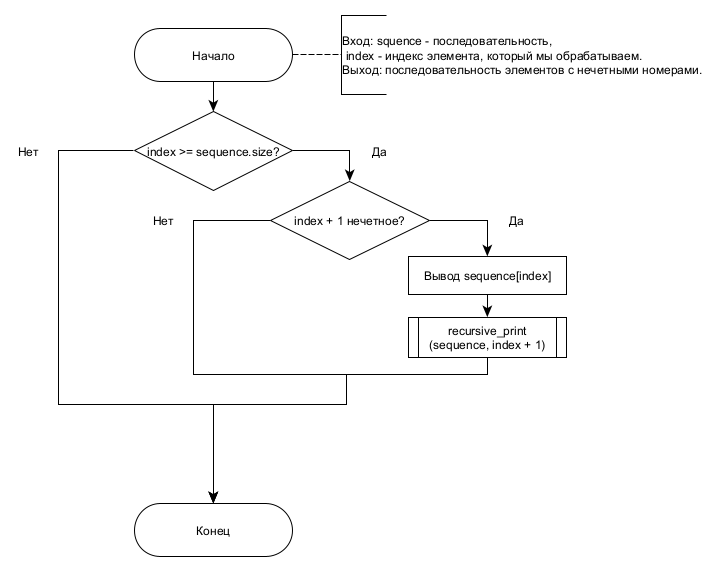
\includegraphics[width=0.9\textwidth, height=0.9\textheight, keepaspectratio]{images/recursive_scheme}
	\caption{Схема рекурсивного алгоритма вывода элементов последовательности с нечетными номерами}
	\label{recursive}
\end{figure}
\clearpage

На рисунке~\ref{iteration} представлена схема итеративного алгоритма вывода элементов последовательности с нечетными номерами.

\begin{figure}[h!]
	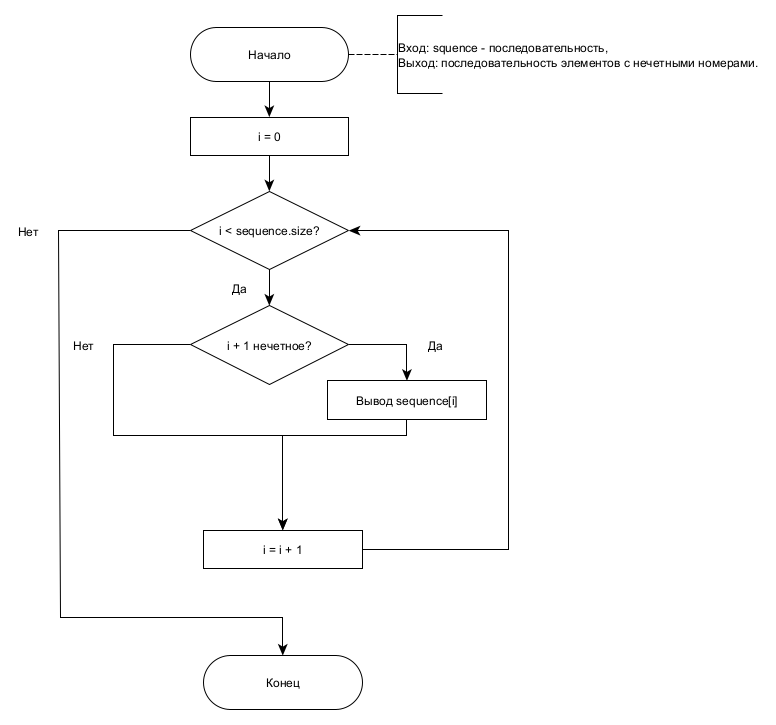
\includegraphics[width=0.9\textwidth, height=0.9\textheight, keepaspectratio]{images/iteration}
	\caption{Схема итеративного алгоритма вывода элементов последовательности с нечетными номерами}
	\label{iteration}
\end{figure}
\clearpage

\section{Теоретическая оценка памяти}
\subsection{Оценка памяти для рекурсивного алгоритма}
Для анализа затрат памяти рекурсивного алгоритма введены следующие обозначения:

\begin{itemize}
	\item $p$ — количество передаваемых параметров (2 параметра);
	\item $r$ — количество сохраняемых регистров (примем 2);
	\item $k$ — количество возвращаемых значений (0);
	\item $l$ — количество локальных переменных (0);
	\item $f$ — ячейка для возвращаемого значения (1).
\end{itemize}

Объем памяти на один фрейм стека рассчитывается по формуле:
\[
f_R(1) = p + k + r + l + f + 1 = 2 + 0 + 2 + 0 + 1 + 1 = 6 \text{ ячеек}
\]

Глубина рекурсии равна количеству вызовов функции, которое зависит от размера входного вектора $n$:
\[
h = n - index_{\text{start}}
\]

В худшем случае (когда $index = 0$):
\[
h = n
\]

Общий объем памяти:
\[
V = f_R(1) \cdot h = 6 \cdot n
\]

Асимптотическая оценка: $O(n)$

\subsection{Оценка памяти для итеративного алгоритма}
Итеративный алгоритм использует фиксированное количество переменных:

\begin{itemize}
	\item входной вектор sequence — 1 переменная (указатель);
	\item счетчик цикла i — 1 переменная.
\end{itemize}

Общий объем памяти постоянен и не зависит от размера входных данных.

Асимптотическая оценка: $O(1)$


\section{Модель вычислений}

Для анализа трудоемкости алгоритмов вводится следующая модель:
\begin{enumerate}
	\item стоимость операций $=, ==, !=, >, <, >=, <=, \&\&, ||, \&=, |=,$ $+=,$ $-=,$ $+,$ $-,$ $[],$ $ ++,$ $--,$ $<<,$ $>>$ принимается равной 1;
	\item стоимость операций $\cdot, /, \cdot=, /=, \%, \%=$ принимается равной 2;
	\item трудоемкость условного оператора вида \textit{if (Условие) \{Блок X\} else \{Блок Y\}}, где вычисление условия и блоков X и Y обозначено как $c_{cond}$, $c_x$, $c_y$, оценивается по формуле~(\ref{if_complexity}):
	\begin{equation}
		\label{if_complexity}
		c_{if} = c_{cond} + 
		\begin{cases}
			\min(c_x, c_y), & \text{лучший случай} \\
			\max(c_x, c_y), & \text{худший случай}
		\end{cases}
	\end{equation}
	\item трудоемкость цикла вида \textit{for (Начало, Условие, Приращение) \{тело\}}, 
	где трудоемкость начальной установки, условия, приращения и тела соответственно 
	равны $c_{start}$, $c_{cond}$, $c_{step}$, $c_{body}$, вычисляется по 
	формуле~(\ref{for_complexity}), где $M$ --- число итераций:
	\begin{equation}
		\label{for_complexity}
		c_{for} = c_{start} + c_{cond} + M \cdot (c_{body} + c_{step} + c_{cond})
	\end{equation}
\end{enumerate}


\section{Оценка трудоемкости алгоритмов}
\subsection{Оценка трудоемкости рекурсивного алгоритма}

Для рекурсивного алгоритма введены обозначения:
\begin{itemize}
	\item $RV(D)$ — количество внутренних вершин дерева рекурсии ($n - 1$);
	\item $RL(D)$ — количество листьев дерева рекурсии (1);
	\item $f_{CV}(1)$ — трудоемкость вычислений во внутренней вершине;
	\item $f_{CL}(1)$ — трудоемкость вычислений в листе.
\end{itemize}

Трудоемкость в листе:
\[
f_{CL}(1) = 1 \text{ (проверка } index \geq sequence.size()) + 0 \text{ (return)} = 1
\]

Трудоемкость во внутренней вершине:
\[
f_{CV}(1) = 1 \text{ (проверка условия)} + 2 \text{ (операция \%)} + 1 \text{ (вывод)} + 1 \text{ (рекурсивный вызов)} = 5
\]

Трудоемкость обслуживания рекурсии на один вызов-возврат:
\[
f_R(1) = 2 \cdot (p + k + l + r + 1 + 1) = 2 \cdot (2 + 0 + 0 + 2 + 2) = 12
\]

Общая трудоемкость:
\begin{align*}
	f_A(n) &= f_R(n) + f_C(n) = R(n) \cdot f_R(1) + [RV(n) \cdot f_{CV}(1) + RL(n) \cdot f_{CL}(1)] \\
	&= n \cdot 12 + [(n - 1) \cdot 5 + 1 \cdot 1] \\
	&= 12n + 5n - 5 + 1 = 17n - 4
\end{align*}

Асимптотическая оценка: $O(n)$

\subsection{Оценка трудоемкости итеративного алгоритма}

Трудоемкость одной итерации цикла:
\[
f_{iteration} = 1 \text{ (проверка } i < sequence.size()) + 2 \text{ (операция \%)} + 1 \text{ (вывод)} + 1 \text{ (инкремент)} = 5
\]

Общая трудоемкость:
\[
f_A(n) = n \cdot f_{iteration} = 5n
\]

Асимптотическая оценка: $O(n)$

\subsection{Сравнительный анализ}

Оба алгоритма имеют линейную временную сложность $O(n)$, где $n$ — размер входного вектора.

\begin{itemize}
	\item \textbf{Рекурсивный алгоритм}: $17n - 4$ операций.
	\item \textbf{Итеративный алгоритм}: $5n$ операций.
\end{itemize}

\section*{Вывод}

В данном разделе были представлены схемы алгоритмов вывода элементов последовательности с нечетными номерами (рисунки 2.1, 2.2), а также была рассчитана теоретическая оценка трудоемкости и памяти.

Теоретический анализ показал, что оба алгоритма имеют линейную временную сложность $O(n)$, где $n$ — размер входной последовательности. Однако наблюдается значительная разница в эффективности:

\begin{itemize}
	\item \textbf{рекурсивный алгоритм} требует $17n - 4$ операций и потребляет $O(n)$ памяти из-за накладных расходов на организацию стека вызовов.
	\item \textbf{итеративный алгоритм} требует всего $5n$ операций и имеет константную сложность по памяти $O(1)$.
\end{itemize}

\textbf{Сравнительный анализ} демонстрирует, что итеративный алгоритм превосходит рекурсивный как по временной эффективности (в 3.4 раза меньше операций), так и по использованию памяти. Рекурсивный подход уступает из-за затрат на создание и уничтожение стековых фреймов для каждого вызова функции.

Для практического применения рекомендуется использовать итеративный алгоритм как более эффективный по ресурсам. Рекурсивный вариант может быть рассмотрен в учебных целях или в случаях, когда ясность кода важнее производительности.